\documentclass[11pt]{article}

\usepackage{wrapfig}
\usepackage{setspace,lipsum}

\usepackage{deauthor,times,graphicx}
\usepackage{color}
\usepackage{eurosym}
\newcommand{\biggorilla}{\mbox{\sc BigGorilla}}
\newcommand{\koko}{\mbox{\sc Koko}}
\newcommand{\flexmatcher}{\mbox{\sc FlexMatcher}}
\newcommand{\magellan}{\mbox{\sc Magellan}}

\newcommand{\tanedit}[1]{{\small \color{blue}~#1}}
\newcommand{\alonedit}[1]{{\small \color{blue}#1}}
\newcommand{\anhaiedit}[1]{{\small \color{blue}#1}}
\newcommand{\spanstr}[1]{{``{\em\small #1}''}}
\newcommand{\token}[1]{\mbox{\rm #1}}
\newcommand{\pystr}{\mbox{\sc py\_stringmatching}}
\newcommand{\pyssj}{\mbox{\sc py\_stringsimjoin}}
\newcommand{\mg}{\mbox{\sc Magellan}}
\newcommand{\where}{\mbox{\sf where}}
\newcommand{\extract}{\mbox{\sf extract}}
\newcommand{\similarTo}{\mbox{\sf similarTo}}
\newcommand{\from}{\mbox{\sf from}}
\newcommand{\ifclause}{\mbox{\sf if}}
\newcommand{\satisfying}{\mbox{\sf satisfying}}
\newcommand{\withthreshold}{\mbox{\sf with threshold}}
\newcommand{\eqclause}{\mbox{\sf eq}}
\newcommand{\inclause}{\mbox{\sf in}}
\newcommand{\orclause}{\mbox{\sf or}}
\newcommand{\excluding}{\mbox{\sf excluding}}
\newcommand{\near}{\mbox{\sf near}}
\newcommand{\contains}{\mbox{\sf contains}}
\newcommand{\mentions}{\mbox{\sf mentions}}
\newcommand{\matches}{\mbox{\sf matches}}
\newcommand{\alt}{\mbox{\sf or}}
\newcommand{\desc}[1]{\{\mbox{\em #1}\}}
\newcommand{\posverb}{\mbox{\sc verb}}
\newcommand{\w}[1]{\mbox{\{{\em #1}\}}}
\newcommand{\descriptor}[1]{\mbox{$[[$#1$]]$}}
\newcommand{\dm}{\mbox{\sc DeepMatcher}}




%\author{ Alon Halevy}


\begin{document}
%\title{The Ubiquity of Subjectivity}
%\maketitle

\begin{abstract}
In order to make effective use of data in decision making, we need to consider aspects of data that our research community has traditionally ignored.  These include the management of subjective data, building unbiased presentations that are tailored to the subjective world-view of the recipient, and finally, the subjective nature of human decision making.
\end{abstract}

\section{Introduction}

Data has become an integral part of our lives. We use data to make a wide spectrum of decisions, such as what to wear today, where to go for dinner and on vacation,  which charity to support, and who to vote for in the elections. Ideally, we'd like to think that if we just had all the facts,  decisions would be easy and disagreements would be quickly settled. As a research community, our goal has been to fuel such decision making by  focusing on  extracting, managing, querying and visualizing data and facts.  I argue here that we need to acknowledge the subjective aspects of data and decision making and broaden our agenda to incorporate them into the systems we build.  

Subjectivity is prevalent in at least three levels. First, the data itself may be subjective: there is no ground truth about whether a restaurant is romantic or a travel destination is relaxing. We need to develop techniques to extract, manage and query subjective data. Second, presentation of the data can be subjective either by introducing bias (intentionally or not), or by tailoring the presentation to the frame of mind of the recipient. Third, human decision making is inherently subjective and based on emotions. We need to understand how to incorporate the emotional aspect of decision making into our systems.  

The following sections will expand on each of these topics.  I have already done some research on the first topic~\cite{subjectivedatabases} and so my comments will be more concrete. However, I believe all three areas are equally important.

\section{Subjective data}
When we compare between multiple options (e.g., hotels, restaurants, online courses), we typically lean on subjective data that describes the {\em experiential aspects} of these options. Today, this data resides in online reviews. For example, reviews will give insights on whether a restaurant has a quiet ambience,   
a hotel has helpful staff, or a school has good faculty. While today's online shopping sites make significant attempts at surfacing key quotes from reviews and even classifying them into several categories, a user cannot put these conditions in the query  (e.g., {\em hotels up to \$250 a night with helpful staff}). Hence, we end up sifting through many reviews until we get exhausted and settle for sub-optimal choices. 

Database systems traditionally focus on the {\em objective} attributes of entities (e.g., the price and location of a hotel, or the cuisine of a restaurant). One exception, which captures a narrow aspect of subjective data, is modeling reviewers' opinions as star ratings, and letting users query the aggregate ratings. 
Subjective data introduces additional technial challenges because it is expressed in free text, is very nuanced, and  does not lend itself to a clean schema.   
The Natural Language Processing  (NLP) community has spent significant effort on subjective data. That community investigated problems such as identifying subjective data~\cite{DBLP:journals/coling/WiebeWBBM04}, studying how subjectivity affects the meaning of words~\cite{DBLP:conf/acl/WiebeM06}, learning extraction patterns for it~\cite{DBLP:journals/taffco/WiebeR11}, and creating summaries of online reviews~\cite{liu2012sentiment}.   Management of subjective data presents an interesting opportunity to combine techniques from databases and NLP.

The first challenge involving subjective data is answering complex queries. 
Roughly speaking, from a query processing perspective, the NLP community has addressed the problem of retrieving individual facts (e.g., finding comments about the friendliness of the hotel staff).  However, to answer more complex queries, a system needs to be able to combine multiple query predicates and to aggregate opinions across many reviews. Combining multiple subjective predicates (e.g., {\em hotels with quiet rooms and friendly staff}) is similar in spirit to the problem of combining multiple sources of fuzzy information~\cite{fagin1996combining}.  
Aggregating subjective data is crucial because users typically want to get an overview of the reviews at hand. The problem of aggregating reviews is fascinating because it requires mapping textual expressions to some meaningful scale. 

The second challenge regarding subjective data is that the schema is much more fluid. Since experiential aspects of an entity can be extremely varied and nuanced, it's not clear which of them to include in the schema. Some attributes may be related to each other or mostly determined by others (e.g., {\sc friendlyStaff} and {\sc helpfulStaff}). Hence, a subjective database system cannot assume that every query it receives can be answered with its schema. In some cases, it will need to find attributes in the schema that are closest to the query terms. In other cases, when the system has low confidence that the schema can be used to answer the query, it will need to fall back on the actual text in the reviews. In some ways, this challenge is similar to how web search engines straddle the boundary between structured and unstructured data.  When a search engine can confidently map a query to an entity in their knowledge graph, the engine presents a knowledge card with structured data.  When the engine thinks the answer appears in a paragraph or an HTML table on the Web, they present that result prominently. But when both of these fail, they fall back on links to ranked Web pages.  


Finally, at the core of the subjective evaluation of data is also the subjective view of the user asking the query.
A hotel that would be considered clean for one person may not cut it for another, and obviously the same goes for cafes. 
Hence, when  user profiles are available, a subjective database should tailor its answers to the user.
 User profiles may be collected passively from previous queries, clicks or purchases, or they may be constructed by answering a few survey questions.
 The next two sections dive deeper into the topic of the user perception. 

\section{Subjective presentation}
To be useful in decision making, data needs to be communicated to a user either textually, orally or visually.  There are two dimensions to subjectivity in the presentation: {\em faithfulness}--whether the data is presented  without bias, and {\em effectiveness}--whether the data is presented in a way that is likely to resonate with the frame of mind of the recipient.

In terms of faithfulness, there are several common methods to create a misleading presentation, including 
 omission, alluding to the {\em straight-line instinct}, and improper comparison~\cite{factfulness}. An example of omission is in Figure~\ref{fig:fig}(a) showing that unemployment rates in the US have been going down since Donald Trump took office in January, 2017, whereas Figure~\ref{fig:fig}(b)  shows that it is merely a continuation of the trend that began during the previous administration. An example of alluding to the straight-line instinct would be to show the world population growth graph in Figure~\ref{fig:fig}(c) and letting the readers extrapolate that it will grow indefinitely. In fact, the common estimates show that the world population will actually peak around 2050. An example of improper comparison would be to state that the GDP of the USA grew by 2.3\% in 2017 but without presenting growth numbers for comparable economies. Note that in some cases search engines already show comparable points when presenting structured data. 

\begin{figure}
\subfloat[a]{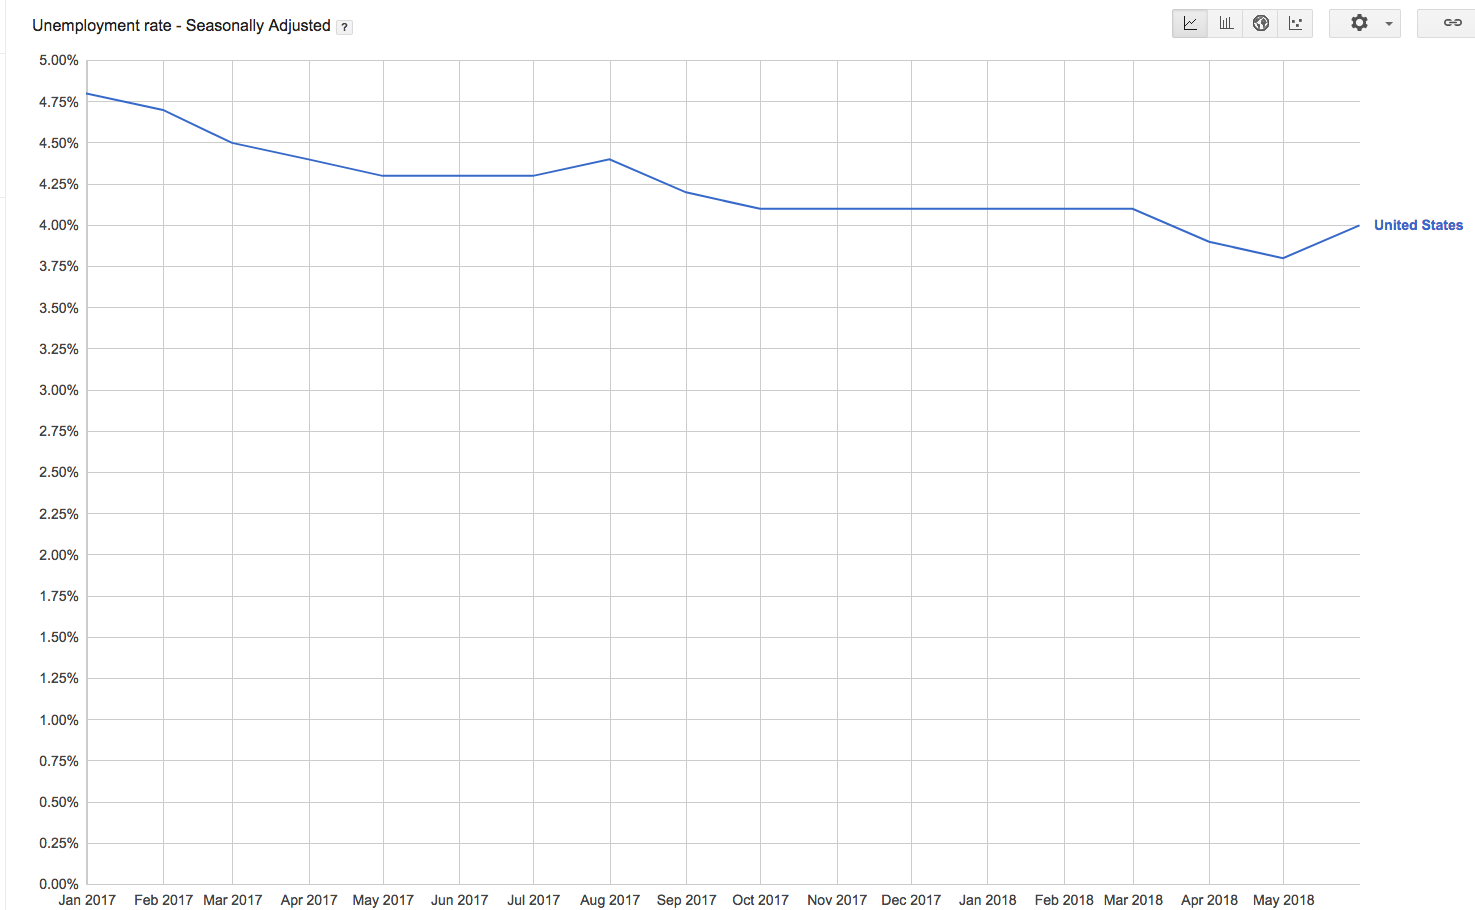
\includegraphics[width = 1.7in]{letters/unemp2017.png}}
\subfloat[b]{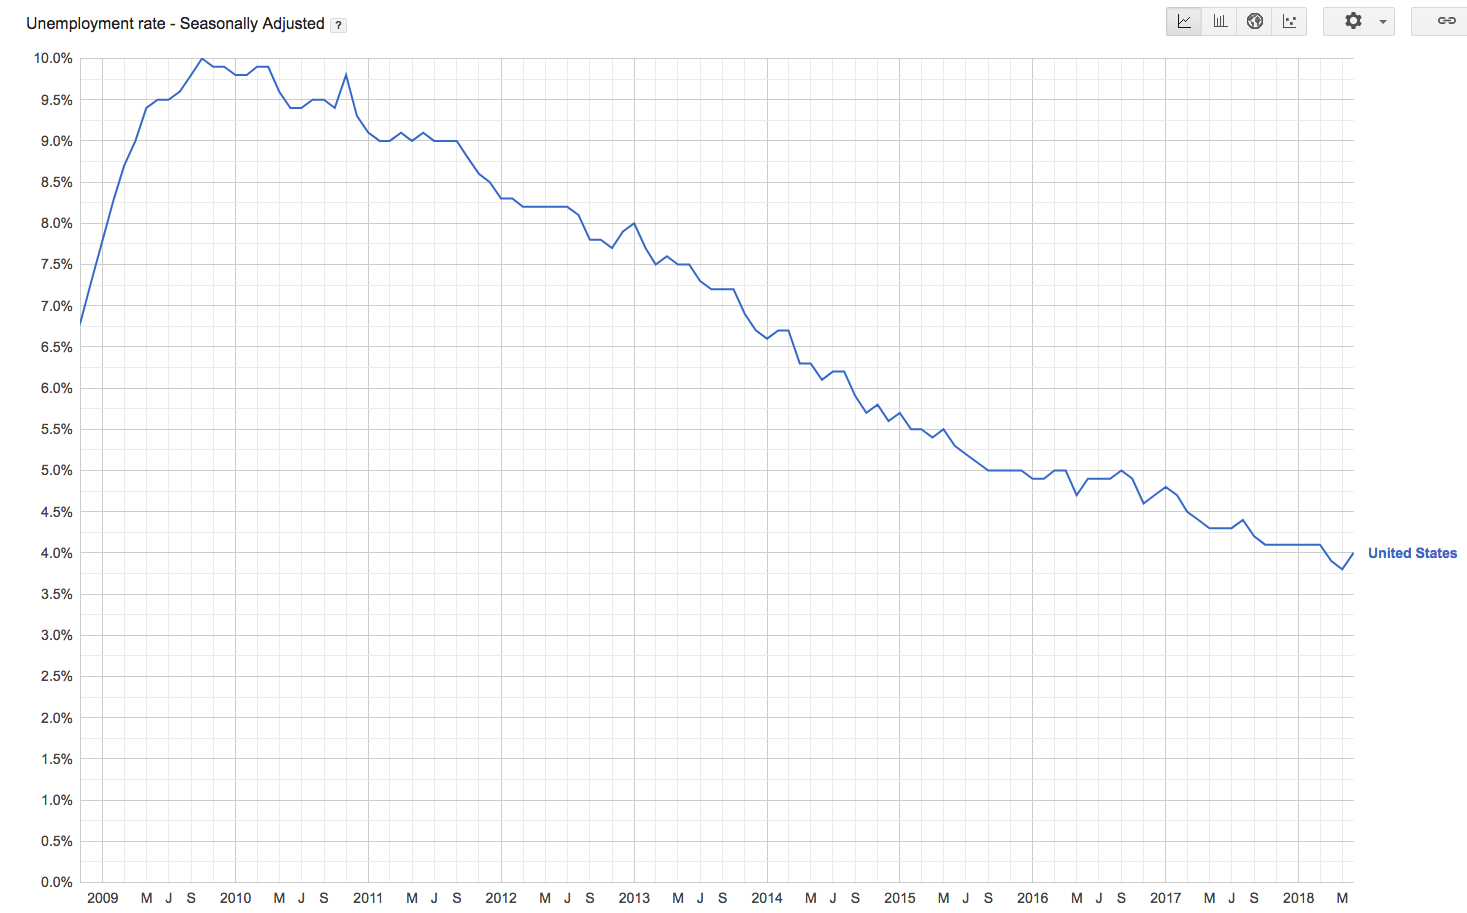
\includegraphics[width = 1.7in]{letters/unemp2009.png}}
\subfloat[c]{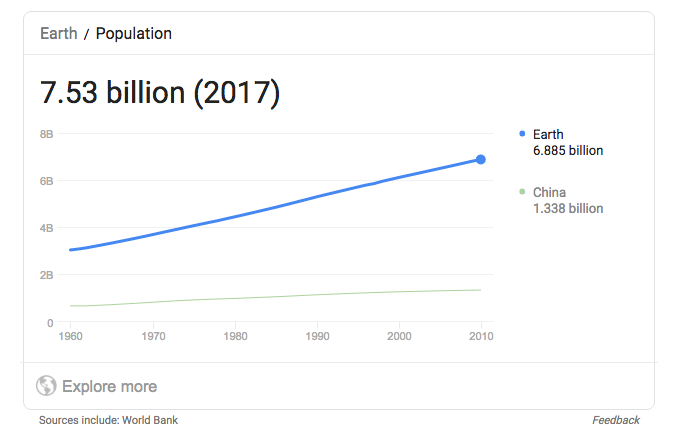
\includegraphics[width = 1.7in]{letters/worldpop.png}} 

\caption{(a) is the unemployment rate in the USA since 2017 and (b) is the rate since 2009. (c) is the world population over time.}
\label{fig:fig}
\end{figure}

In the above examples the presenter seems at least slightly nefarious by hiding relevant aspects of the data (see~\cite{DBLP:conf/edbt/StoyanovichAM16} for a more detailed discussion of fairness in data analysis). But subjectivity in presentation can also be done in trying to frame data in a way that can resonate better with the recipient. Such a presentation could make the difference between making a convincing case or falling on flat ears. Lakoff and Wehling discuss the framing issue  in the context of political debates~\cite{lakoff-book}. They discuss the example of the healthcare debate in American politics and claim that once the healthcare is framed as a product, there is little chance of convincing conservatives that it should be available to everyone and that everyone should be forced to buy healthcare. After all, a government should not force its citizens to buy {\em any} product, be it peanut butter, striped socks, or healthcare? In contrast, if healthcare is framed as an issue of freedom, which is central to the conservative doctrine, then conservatives would see the merits. After all, you are not truly free if a medical condition can completely deplete all your assets.   

The above discussion leads to several research problems: 
(1) {\em is $P$ a faithful presentation of the data $D$?} (2) {\em Does a presentation $P$ of data $D$ support an argument $A$}?  (3) {\em is the presentation $P$ of data $D$ effective for the user $U$?} Note that effectiveness is different from relevance--data can be relevant, but the user may still ignore it if not presented effectively. In a particular context, these problems will be made more specific. For example, we will have some space of possible presentations (e.g., graphs spanning different time periods), and for elements of that space we can consider specific questions, such as would a presentation of a graph of a variable over time incorrectly lead to inducing wrong conclusions with the straight line instinct? Could one falsely conclude a particular pattern without looking at a broader time scale?  What are appropriate comparison points for a particular datum? 

\section{Subjective decision making}
We would like to think that our decision making is rational and based on hard facts. In practice, however, it is well known from psychology and Neuroscience that our emotions, which express many of our subjective preferences, play a large part in our decision making~\cite{kahneman}. In fact, it has been shown that {\em without} emotions we cannot make even simple decisions. A famous case in point was Antonio Damasio's patient named Elliot~\cite{damasio}. Elliot suffered a particular type of damage to his brain following the removal of a tumor and was unable to feel any emotion, even when he was shown very disturbing images. While Elliot's IQ remained in tact, he was not able to make simple decisions such as how to prioritize work items or choose an item from a restaurant menu.


I am not suggesting that the intricacies of decision making can be reformulated as a data management problem, but I think we can do a much better job at incorporating the emotional aspect of decision making into the systems we build.\footnote{Rosalind Picard already pointed in this direction in 1997 in her original book on Affective Computing~\cite{picard-book}, (page 220).} 
From a computational perspective, decision making involves exploring a large state space of possible outcomes, such as choosing a hotel to stay during a trip, or the best method for securing child care for your baby. The first challenge to decision making arises because the number of possible states may be too large to consider,  especially under time and attention pressure. Second, we may have incomplete or only probabilistic knowledge about these possible states, making the comparison even sketchier. Finally, many of the choices we make in life (e.g., between job offers or romantic prospects) are not really directly comparable  to each other.

To reach decisions effectively, we prune the search space using heuristics that may not be conscious (e.g., certain attributes of entities end up being more important under certain conditions). Developing an understanding of how we prune the decision search space and methods that result in better decisions presents an exciting area of research that our current data science tool set is well poised to investigate.

\section{Conclusion}
To  realize the full potential of the vast amounts of data available to us today, systems need to be able to manage subjective data and to understand how prospective consumers of the data think and make decisions subjectively. I've tried to outline a few concrete steps on this research agenda. Of course, as we tackle these problems, we should also keep in mind that ultimately the data we have is merely an abstraction of the world and there will be other factors that are not included in the data that will influence our decisions and actions. In a nutshell, this is a call to consider concepts from psychology, behavior economics and neuroscience in the design of tools that enable decision making based on data. 

\section{Acknowledgements}
I'd like to thank my colleagues at Megagon Labs for inspiring many of the ideas described above: Wang-Chiew Tan, Vivian Li, Adi Zief-Balteriski, Yuliang Li and Jingfeng Li. Thanks to Phil Bernstein,  Anna-Lisa Gentile, Rada Mihalcea and Haixun Wang for several discussions relating to the topics covered.


%\scriptsize
%\newpage
\vspace{-.1cm}
\bibliographystyle{ACM-Reference-Format}
\begin{thebibliography}{10}
\begin{small}



\itemsep=-.5pt

\bibitem{damasio}
A.~Damasio.
\newblock {\em Descartes' Error}.
\newblock Springer, 1994.

\bibitem{fagin1996combining}
R.~Fagin.
\newblock Combining fuzzy information from multiple systems.
\newblock In {\em PODS}, pages 216--226. ACM, 1996.

\bibitem{kahneman}
D.~Kahnnman.
\newblock {\em Thinking Fast and Slow}.
\newblock Penguin Books, 2012.

\bibitem{lakoff-book}
G.~Lakoff and E.~Wehling.
\newblock {\em The Little Blue Book: The Essential Guide to Thinking and
  Talking Democratic}.
\newblock Free Press, 2012.

\bibitem{subjectivedatabases}
Y.~Li, J.~Li, A.~Feng, V.~Li, W.-C. Tan, and A.~Halevy.
\newblock Subjective databases.
\newblock {\em arXiv preprint arXiv:1309.0238}, 2019.

\bibitem{liu2012sentiment}
B.~Liu.
\newblock {\em Sentiment Analysis and Opinion Mining}.
\newblock {Morgan & Claypool}, 2012.

\bibitem{picard-book}
R.~Picard.
\newblock {\em Affective Computing}.
\newblock The M.I.T Press, 1995.

\bibitem{factfulness}
H.~Rosling, O.~Rosling, and A.~R. Rönnlund.
\newblock {\em Factfulness: Ten Reasons We're Wrong About the World--and Why
  Things Are Better Than You Think}.
\newblock Flatiron Books, 2018.

\bibitem{DBLP:conf/edbt/StoyanovichAM16}
J.~Stoyanovich, S.~Abiteboul, and G.~Miklau.
\newblock Data responsibly: Fairness, neutrality and transparency in data
  analysis.
\newblock In E.~Pitoura, S.~Maabout, G.~Koutrika, A.~Marian, L.~Tanca,
  I.~Manolescu, and K.~Stefanidis, editors, {\em Proceedings of the 19th
  International Conference on Extending Database Technology, {EDBT} 2016,
  Bordeaux, France, March 15-16, 2016, Bordeaux, France, March 15-16, 2016.},
  pages 718--719. OpenProceedings.org, 2016.

\bibitem{DBLP:conf/acl/WiebeM06}
J.~Wiebe and R.~Mihalcea.
\newblock Word sense and subjectivity.
\newblock In N.~Calzolari, C.~Cardie, and P.~Isabelle, editors, {\em {ACL}
  2006, 21st International Conference on Computational Linguistics and 44th
  Annual Meeting of the Association for Computational Linguistics, Proceedings
  of the Conference, Sydney, Australia, 17-21 July 2006}. The Association for
  Computer Linguistics, 2006.

\bibitem{DBLP:journals/taffco/WiebeR11}
J.~Wiebe and E.~Riloff.
\newblock Finding mutual benefit between subjectivity analysis and information
  extraction.
\newblock {\em {IEEE} Trans. Affective Computing}, 2(4):175--191, 2011.

\bibitem{DBLP:journals/coling/WiebeWBBM04}
J.~Wiebe, T.~Wilson, R.~F. Bruce, M.~Bell, and M.~Martin.
\newblock Learning subjective language.
\newblock {\em Computational Linguistics}, 30(3):277--308, 2004.

\end{thebibliography}



\end{document}
